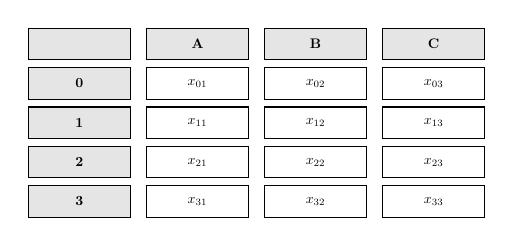
\begin{tikzpicture}[scale=0.5, transform shape,
    cell/.style={
        draw,
        minimum width=2.6cm,
        minimum height=0.8cm,
        align=center
    },
    header/.style={
        cell,
        fill=gray!20,
        font=\bfseries
    },
    highlight/.style={
        cell,
        fill=blue!15
    }
]

%------------------------------------------------
% Parámetros
%------------------------------------------------
\def\ncols{3}
\def\nrows{4}
\def\xstep{3}
\def\ystep{1}

%------------------------------------------------
% Encabezados de columnas
%------------------------------------------------
\node[header] at (0,0) {}; % esquina vacía

\foreach \j/\name in {1/A,2/B,3/C} {
    \node[header] at (\j*\xstep,0) {\name};
}

%------------------------------------------------
% Filas del DataFrame
%------------------------------------------------
\foreach \i in {0,...,3} {

    % índice
    \node[header] at (0,-\i*\ystep-\ystep) {\i};

    % celdas
    \foreach \j in {1,...,3} {
        \node[cell] at (\j*\xstep,-\i*\ystep-\ystep)
        {$x_{\i\j}$};
    }
}

\end{tikzpicture}
